\documentclass[main.tex]{subfiles}
\begin{document}
\section{Colourings}
\begin{definition*}[Proper colouring, $\chi(G)$, $k$-colouring]
  A colouring $c:V(G)\to C$ is \vocab[proper colouring]{proper} if
  $x\sim_G y\implies c(x)\neq c(y)$.

  {\color{blue}$\chi(G)$} is the minimum $k$ such that $G$ has a
  \vocab[k-colouring@\2]{$k$-colouring}, i.e. a proper colouring where $|C| = k$.
\end{definition*}
We have the following generalization of graph colouring.
\begin{definition*}[List assignment, $k$-list-assignment, $L$-colouring, list chromatic number]
  \listhack
  \begin{itemize}
    \item A \vocab{list assignment} $L$ of $G$ is a function $L:V(G)\to 2^\bN$.
    \item $L$ is a \vocab[list assignment!k-list-assignment@\2]{$k$-list-assignment}
      if $|L(v)|\geq k$ for all $v$.

    \item An \vocab[L-colouring@\2]{$L$-colouring} of $G$ is a proper colouring
      $c$ of $G$ such that $c(v)\in L(v)$ for all $v\in V(G)$.

    \item The \vocab{list chromatic number} $\chi_\ell(G)$ is the minimum $k$
      such that for every $k$-list-assignment $L$ of $G$, there is an
      $L$-colouring of $G$.
  \end{itemize}
\end{definition*}
Note that $\chi_\ell(G)\geq\chi(G)$.
This is because if $k < \chi(G)$ the constant $k$-list-assignment $L$ with
$L(v) = \{1,\ldots,k\}$ for all $v$ is a $k$-list-assignment.

\begin{example*}
  Consider the graph $G$:
  \begin{center}
    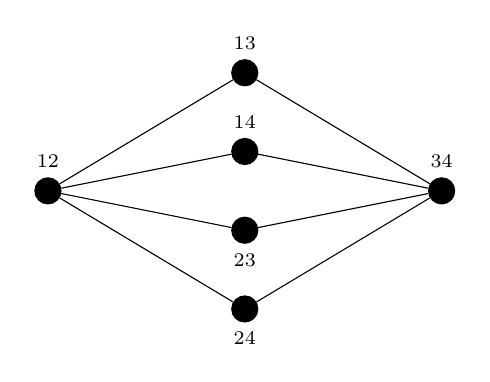
\begin{tikzpicture}
      \node[draw, fill=black, circle, label=above:{\scriptsize 12}] (a) at (-2.5,0) {};
      \node[draw, fill=black, circle, label=above:{\scriptsize 13}] (c) at (0,1.5) {};
      \node[draw, fill=black, circle, label=above:{\scriptsize 14}] (d) at (0,0.5) {};
      \node[draw, fill=black, circle, label=below:{\scriptsize 23}] (e) at (0,-0.5) {};
      \node[draw, fill=black, circle, label=below:{\scriptsize 24}] (f) at (0,-1.5) {};
      \node[draw, fill=black, circle, label=above:{\scriptsize 34}] (b) at (2.5,0) {};
      \draw (a) -- (c) -- (b);
      \draw (a) -- (d) -- (b);
      \draw (a) -- (e) -- (b);
      \draw (a) -- (f) -- (b);
    \end{tikzpicture}
  \end{center}
  Note $\chi(G) = 2$ as it is bipartite, but $\chi_\ell(G) > 2$ because
  $G$ has no $L$-colouring for the indicated $L$.
  (It turns out the list chromatic number of this graph is 3.)
\end{example*}
We can however bound the list chromatic number (and thus the chromatic number).
\begin{definition*}[$d$-degenerate]
  $G$ is \vocab[d-degenerate@\2]{$d$-degenerate} if every non-empty subgraph of
  $G$ has a vertex of degree $\leq d$.
\end{definition*}
Note that $d$-degeneracy is related to (but not equivalent to!) minimum degree,
as $d$-degeneracy holds under taking subgraphs, but minimum degree does not.
\begin{proposition}
  If $G$ is $d$-degenerate, then $\chi_\ell(G)\leq d+1$.
\end{proposition}
\begin{proof}
  Induct on $n = v(G)$.
  If $n = 1$, the result follows trivially; otherwise $L$ be a $(d+1)$-list
  assignment and $v$ be a vertex of degree at most $d$ in $G$.
  \lecture{Thu Oct 26}%
  Inductively, $G-v$ has an $L$-colouring $c_0$.
  Then
  \begin{align*}
    |L(v)\setminus\{c_0(x) : x\sim v\}| &\geq|L(v)\setminus N_G(v)| \\
                                        &\geq |L(v)| - d > 0.
  \end{align*}
  So there exists $k\in L(v)$ that was not assigned by $c_0$ to any neighbour
  of $v$.
  Extending $c_0$ by assigning $k$ to $v$ gives an $L$-colouring of $G$.
\end{proof}
\begin{remark*}
  \listhack
  \begin{itemize}
    \item This is similar to the 6-colouring proof of planar graphs,
      because planar graphs are 5-degenerate.

    \item The name ``$d$-degenerate'' comes from there being an ordering of
      the vertices such that each vertex has backwards degree at most $d$.
  \end{itemize}
\end{remark*}
There are a couple of consequences of this degeneracy bound.
\begin{corollary}
  \listhack
  \begin{itemize}
    \item $\chi(G)\leq\chi_\ell(G)\leq\max_{\varnothing\neq H\subseteq G}\delta(H) + 1$;

    \item $\chi_\ell(G)\leq\max_{\varnothing\neq H\subseteq G}
      \left(\frac{2e(H)}{|V(H)|}\right)+1$; \mnote{The expression inside the
        max is the average degree of $H$, and the overall expression is called
      \textit{maximum average degree.}}

    \item $\chi_\ell(G)\leq\Delta(G) + 1$.
  \end{itemize}
\end{corollary}
The latter bound is tight for complete graphs and odd cycles;
we will prove later these are the only graphs where the bound is tight.

\begin{theorem} \rmnote{This implies $\chi_\ell(G)$ and $\chi(G)$ are not
  qualitatively related, i.e. it is not the case that if one goes
  to infinity, the other will also go to infinity.}%
  For all $t$, there is a graph $G$ with $\chi(G) = 2$ and $\chi_\ell(G) > t$.
\end{theorem}
\begin{proof}
  Given $t$, let $c_1,\ldots,c_t$ be disjoint $t$-sets in $\bN$.
  Let $G\cong K_{t,t^t}$ have bipartition $(A,B)$ where $A = \{a_1,\ldots,a_t\}$
  and $|B| = t^t$.
  Let $L$ be a $t$-list assignment of $G$ such that $L(a_i) = c_i$ and the lists
  assigned to the vertices in $B$ are precisely the elements of
  $U = \{\{x_1,\ldots,x_t\} : x_i\in c_i\;\forall i\}$ (and since $|U| = t^t$,
  this is possible).

  If $c$ is an $L$-colouring of $G$, then $\{c(a_1),\ldots,c(a_t)\}\in U$
  so there is a vertex $b\in B$ such that $L(b) = \{c(a_1), \ldots, c(a_t)\}$.
  But this means $c(b) = c(a_i)$ for some $i$, contradicting $a_i\sim b$.
\end{proof}

\begin{theorem}[Brooks' Theorem]\mnote{This proof adapts fairly nicely to
  $\chi_\ell(G)\leq\Delta(G)$.}
  If $G$ is connected, then $\chi(G)\leq\Delta(G)$ \underline{unless} $G$ is
  a complete graph or an odd cycle.
\end{theorem}
\begin{proof}[Proof (Zajac '18)]
  It suffices to show:
  \begin{enumerate}[label=(\arabic*)]
    \item If $t\geq 3$ and $\Delta(G)\leq t$ and $G$ has no $K_{t+1}$ subgraph,
      then $\chi(G)\leq t$.
      \rmnote{$t\geq 3$ to deal with odd cycles;
      this statement also holds for $\chi_\ell(G)$.}
  \end{enumerate}
  We use the following key lemma.
  \begin{lemma}
    Let $\Delta(G)\leq t$, and $x$ be an end vertex of a path $P$ of $G$.
    Then every $t$-colouring $c_0$ of $G - V(P)$ extends to a $t$-colouring
    of $G - x$.
  \end{lemma}
  \begin{subproof}
    \mnote{There might be a cleaner proof based on inducting on $|P|$.}%
    Let $v_1,\ldots,v_k = x$ be the vertices of $P$.
    For each $i$, let $G_i = G[(G - V(P))\cup\{v_1,\ldots,v_i\}]$.
    We want to show that $c_0$ extends to a $t$-colouring of $G_{k-1} = G - x$.
    Let $i\in\{0,\ldots,k-1\}$ be maximal such that $c_0$ extends to a
    $t$-colouring $c_i$ of $G_i$.
    If $i = k-1$, we're done.
    Otherwise, $i\leq k-2$.

    Since $v_{i+1}$ has the neighbour $v_{i+2}\notin V(G_i)$, the vertex
    $v_{i+1}$ has at most $t-1$ neighbours in $G_i$, so there is some colour
    $\kappa$ not assigned by $c_i$ to any neighbour of $v_{i+1}$.
    But then assigning $\kappa$ to $v_{i+1}$ extends $c_i$ to a $t$-colouring
    $c_{i+1}$ of $G_{i+1}$, contradicting the maximality of $G_i$.
  \end{subproof}
  Let $G$ be a counterexample to (1) on as few vertices as possible.
  Note:
  \begin{itemize}
    \item $G$ is connected (otherwise, inductively colour its components,
      then combine);

    \item $|V(G)|\geq t+1$ (otherwise it's $t$-colourable);

    \item $G$ is $t$-regular (otherwise, inductively colour $G - v$ for some
      $v$ with degree strictly less than $t$, then extend to a colouring of
      $G$ using an available colour).
  \end{itemize}

  Let $v$ be a vertex.
  Since $d(v) = t$ and $K_{t+1}$ is not a subgraph of $G$, it follows that $v$
  has two non-adjacent neighbours.
  Let $v_1, v_2, \ldots, v_\ell$ be a maximal path of $G$ such that
  $v_1\not\sim v_3$.

  \begin{itemize}
    \item \textbf{Case 1:} $\{v_1,\ldots,v_\ell\} = V(G)$

      \mnote{This needs $V(G) = V(P)$ to work.}
      Since $G$ is $t$-regular for $t\geq 3$, there is a neighbour
      $v_j\notin\{v_1,v_3\}$ of $v_2$.
      Let $c_0$ be a $t$-colouring of $G[\{v_1,v_3\}]$ where $c_0(v_1) = c_0(v_3)$.
      By the lemma applied to the path $\{v_\ell, v_{\ell-1},\ldots,v_j\}$ with
      $x = v_j$, the colouring $c_0$ extends to a $t$-colouring of
      $G[\{v_1,v_3\}\cup\{v_\ell, v_{\ell-1},\ldots,v_{j+1}\}]$.

      By the lemma applied to the path $\{v_4, \ldots, v_j, v_2\}$ with $x = v_2$,
      the colouring $c_1$ extends to a $t$-colouring $c_2$ of
      $G[\{v_1,v_3\}\cup\{v_\ell,\ldots,v_{j+1}\}\cup\{v_4,\ldots,v_j\}] = G - v_2$.

      Now $c_2$ is a $t$-colouring of $G - v_2$ where the neighbours $v_1,v_3$
      of $v_2$ have the same colour.
      Since $d(v_2) = t$, there is a colouring not assigned by $c_2$ to a
      neighbour of $v_2$.
      So $G$ has a $t$-colouring.

    \item \textbf{Case 2:} $\{v_1,\ldots,v_\ell\}\neq V$

      Let $s$ be minimal such that $v_\ell\sim v_s$ for $s < \ell - 1$;
      this exists because $d(v_\ell)\geq 3$.
      Now $C = \{v_s,\ldots,v_\ell\}$ is a cycle containing a vertex (i.e. $v_\ell$)
      with no neighbour outside $C$, and (since $G$ is connected and $V(G)\neq V(C)$),
      a vertex with a neighbour outside of $C$.
      Let $u,v,$ be adjacent in $C$ such that
      $u$ has a neighbour $w$ outside $C$, and $v$ has no neighbour outside $C$.

      Inductively, $G - C$ has a $t$-colouring $c_0$.
      Assign colour $c_0(w)$ to $v$ to get a $t$-colouring $c_1$ of $(G - C) + v$.
      By the lemma applied to the path $C - v$ with $x = u$,
      $c_1$ extends to a $t$-colouring $c_2$ of
      $G[(V(G) - V(C))\cup\{v\}\cup(V(C)\setminus\{u,v\})] = G - u$.
      Now $c_2$ assigns the same colour to neighbours $v,w$ of $u$,
      and so extends to a $t$-colouring of $G$. \qedhere
  \end{itemize}
\end{proof}
\subsection{Colouring Planar Graphs}
\begin{conjecture}[Guthrie 1952]\lecture{Tue Oct 31}%
  Planar graphs are 4-colourable.
\end{conjecture}
Kempe had a false proof in 1879, error found by Heawood.
\begin{theorem}[Heawood 1922]
  Planar graphs are 5-colourable.
\end{theorem}
Proof uses \textit{Kempe chains}.
\begin{theorem}[Appel/Haken 1976]
  Planar graphs are 4-colourable.
\end{theorem}
The idea is to use a technique called ``discharging'' to do the induction,
and the proof involves looking at minimal counterexamples.

In 1996, Robertson, Sanders, Seymour, Thomas came up with a new proof
(but it still requires a complicated reduction to a computation).

There was a formalization by Gonthier in 2008 (mostly likely in Coq).

There is a simpler proof of a 5-colour theorem (using minors).
\begin{proof}[Proof of 5-colour theorem (Seymour)]
  Let $G$ be a minimal counterexample.
  \begin{fact*}[Euler's Theorem]
    \leavevmode\vspace{-0.5em}
    \[
      |V| - |E| + |F| = 1 + c
    \]
    and
    \[
      2|E| = \sum_{f\in F}\deg(f)\geq 3|F|
    \]
    so $|F|\leq\frac 2 3|E|$.
    It follows that $1 + c = |V| - |E| + |F|\leq|V| - \frac 1 3|E|$ so
    $|E|\leq 3|V| - 6$, and the average degree of $G$ is $\frac{2|E|}{|V|} < 6$,
    so every planar graph has a vertex of degree at most 5.
  \end{fact*}
  Let $x$ be a vertex of degree at most 5.
  Inductively, $G - x$ is 5-colourable.
  We may assume that $x$ has 5 neighbours, otherwise we can extend a colouring
  of $G - x$ to a colouring of $G$.

  Let $u,v$ be non-adjacent neighbours of $x$ (such neighbours exist as $K_6$
  is non-planar).
  Let $G_0 = (G - x + uv)/uv$.
  \mnote{Note we are not contracting an edge of the graph, as that can not be
  extended to a colouring of the whole graph.}
  Then $G_0$ is isomorphic to a proper minor of $G$, so is planar.
  So $G_0$ is 5-colourable.
  It follows that $G-x$ has a 5-colouring where $u, v$ have the same colour.
  This extends to a 5-colouring of $G$.
\end{proof}

\begin{theorem}[Grotzsch 1959]
  Triangle-free planar graphs are 3-colourable.
\end{theorem}
\begin{proof}[Proof sketch]
  You can 3-colour an outer cycle and extend to a 3-colouring of the whole graph.
\end{proof}
You can modify the previous proof to easily show triangle-free planar graphs are
4-colourable.
\begin{proof}[Proof Sketch]
  Seymour's proof of the 5-colouring theorem can be modified by strengthening
  the bound to
  \[
    2|E| = \sum_{f\in F}\deg(f)\geq 4|F|
  \]
  (and the result follows).
\end{proof}

\begin{theorem}[Thoamassen 1995]
  Planar graphs are all 5-list-colourable.
\end{theorem}
\begin{proof}
  We will actually prove
  \begin{claim}
    If $G$ is a planar near-triangulation
    (i.e. has a cycle $C$ bounding the infinite face and all other faces are
    bounded by triangles) and $L$ is a list-assignment of $G$ such that
    \begin{itemize}
      \item $|L(v)| = 5$ for all $v\notin V(C)$;
      \item there are $C$-adjacent vertices $x,y$ in $C$ such that $L(x), L(y)$
        are disjoint singletons; and
      \item $|L(v)| = 3$ for all $v\in V(C)\setminus\{x,y\}$
    \end{itemize}
    then $G$ is $L$-colourable.
  \end{claim}
  \begin{subproof}
    Let $G$ be a counterexample with as few vertices as possible.
    \begin{itemize}
      \item \textbf{Case I}: $C$ has a chord (i.e. there are two non-adjacent
        vertices of $C$ joined by an edge of $G$).

        Let $wz$ be a chord of $C$.
        Then $G = G_1\cup G_2$ where $G_1,G_2$ intersect in just the edge $wz$
        and $x,y\in V(G_2)$.
        Let $c_2$ be an $L$-colouring of $G_2$.
        This exists because the unbounded face of $G_2$ is contained in that of
        $G$.

        Let $L'$ be a list assignment of $G_1$ where
        \begin{align*}
          L'(w) &= \{c_2(w)\}, &
          L'(z) &= \{c_2(z)\}, &
          L'(v) &= L(v)\ \text{for all other $v$.}
        \end{align*}
        Since $w, z$ are adjacent vertices on the unbounded face of $G_1$,
        it has an $L'$-colouring $c_1$.
        Combining $c_1, c_2$ gives an $L$-colouring of $G$.

      \item \textbf{Case II:} $G$ has no chord.

        Let $z\neq y$ be adjacent to $x$ on the bounding cycle.
        Then $G - z$ has bounding cycle $(C - z)\cup P$ (this follow by $G$
        being a planar near-triangulation), where $P$ is a path
        from $x$ to the other neighbour $w$ of $z$ in $C$, and $P$ has internal
        vertices outside $C$.
        Let $\kappa, \kappa'$ be distinct colours in $L(z) - L(x)$.
        For each internal vertex $v$ of $P$, let
        $L'(v)\subseteq L(v)\setminus\{\kappa,\kappa'\}$ have size 3.
        For each other vertex $v$ of $G - z$, let $L'(v) = L(v)$.
        Inductively, $G - z$ has an $L'$-colouring.
        Since no neighbours of $z$ in $P$ have colours $\kappa$ or $\kappa'$,
        at least one of $\kappa, \kappa'$ is assigned by $c$ to no vertex in
        $P - x$, nor to $w$.
        Assigning this colour to $z$ gives an $L$-colouring of $G$.
        \qedhere
    \end{itemize}
  \end{subproof}
  \mnote{For assignments, be more precise about the reduction than this.}%
  Note this implies the original theorem, since any 5-list-assignment of a
  planar graph $G$ can be converted to one as in the statement by adding edges,
  and removing colours from lists.
\end{proof}
\begin{theorem}[Voigt 1993]
  There exists a planar graph that is not 4-choosable (i.e. not 4-list-colourable).
\end{theorem}
This counterexample involves around 100 vertices.
\begin{theorem}[Gutner 1996]
  There exists a planar graph that is 3-colourable and not 4-choosable.
\end{theorem}
The example that showed $\chi(\cdot)$ and $\chi_\ell(\cdot)$ can differ
arbitrarily used very disjoint lists, but this is not the case here.
\begin{theorem}[Voight/Wirth 1997]
  There exists a planar graph that is 3-colourable and not 4-choosable,
  even when lists are contained in $\{1,2,3,4,5\}$.
\end{theorem}
There is a nicer counterexample by Mirzalzhani in 1996.
\begin{lemma}
  Define the graph $H_0$ as follows
  \begin{center}
    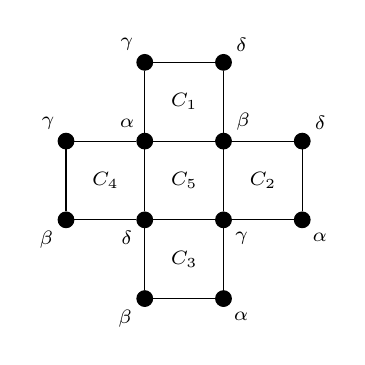
\begin{tikzpicture}[
        scale=0.5,
        every node/.style={draw,fill=black,circle,inner sep=2pt}
      ]
      \node[label=above left:{\scriptsize $\alpha$}] (c5a) at (-1, 1) {};
      \node[label=above right:{\scriptsize $\beta$}] (c5b) at (1, 1) {};
      \node[label=below right:{\scriptsize $\gamma$}] (c5c) at (1, -1) {};
      \node[label=below left:{\scriptsize $\delta$}] (c5d) at (-1, -1) {};
      \node[label=above left:{\scriptsize $\gamma$}] (c4c) at (-3, 1) {};
      \node[label=below left:{\scriptsize $\beta$}] (c4b) at (-3, -1) {};
      \node[label=below right:{\scriptsize $\alpha$}] (c3a) at (1, -3) {};
      \node[label=below left:{\scriptsize $\beta$}] (c3b) at (-1, -3) {};
      \node[label=above right:{\scriptsize $\delta$}] (c2d) at (3, 1) {};
      \node[label=below right:{\scriptsize $\alpha$}] (c2a) at (3, -1) {};
      \node[label=above right:{\scriptsize $\delta$}] (c1d) at (1, 3) {};
      \node[label=above left:{\scriptsize $\gamma$}] (c1c) at (-1, 3) {};
      \draw (c5a) -- (c5b) -- (c5c) -- (c5d) -- (c5a);
      \draw (c5a) -- (c5d) -- (c4b) -- (c4c) -- (c5a);
      \draw (c5c) -- (c3a) -- (c3b) -- (c5d) -- (c5c);
      \draw (c5b) -- (c2d) -- (c2a) -- (c5c) -- (c5b);
      \draw (c5b) -- (c1d) -- (c1c) -- (c5a) -- (c5b);
      \node[draw=none,fill=none] at (0, 0) {\scriptsize $C_5$};
      \node[draw=none,fill=none] at (-2, 0) {\scriptsize $C_4$};
      \node[draw=none,fill=none] at (0, -2) {\scriptsize $C_3$};
      \node[draw=none,fill=none] at (2, 0) {\scriptsize $C_2$};
      \node[draw=none,fill=none] at (0, 2) {\scriptsize $C_1$};
    \end{tikzpicture}
  \end{center}
  with function $f_0:V(H_0)\to\{\alpha,\beta,\gamma,\delta\}$.

  For any proper colouring $c:V(H_0)\to\{\alpha,\beta,\gamma,\delta\}$ with
  $c(x)\neq f_0(x)$ for all $x$, some 4-cycle $C_i$ contains all four colours.
\end{lemma}
\begin{proof}
  Suppose not, so $c$ has two diagonal vertices of the same colour in each $C_i$.
  By case analysis, the result follows.
\end{proof}
\begin{lemma}
  Define the graph $H_1$ as follows
  \begin{center}
    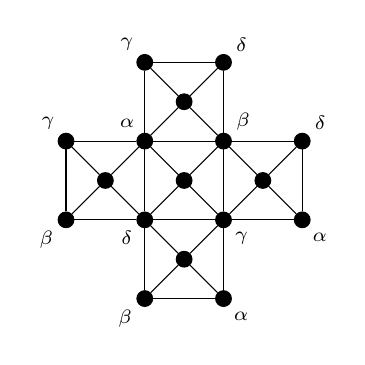
\begin{tikzpicture}[
        scale=0.5,
        every node/.style={draw,fill=black,circle,inner sep=2pt}
      ]
      \node[label=above left:{\scriptsize $\alpha$}] (c5a) at (-1, 1) {};
      \node[label=above right:{\scriptsize $\beta$}] (c5b) at (1, 1) {};
      \node[label=below right:{\scriptsize $\gamma$}] (c5c) at (1, -1) {};
      \node[label=below left:{\scriptsize $\delta$}] (c5d) at (-1, -1) {};
      \node[label=above left:{\scriptsize $\gamma$}] (c4c) at (-3, 1) {};
      \node[label=below left:{\scriptsize $\beta$}] (c4b) at (-3, -1) {};
      \node[label=below right:{\scriptsize $\alpha$}] (c3a) at (1, -3) {};
      \node[label=below left:{\scriptsize $\beta$}] (c3b) at (-1, -3) {};
      \node[label=above right:{\scriptsize $\delta$}] (c2d) at (3, 1) {};
      \node[label=below right:{\scriptsize $\alpha$}] (c2a) at (3, -1) {};
      \node[label=above right:{\scriptsize $\delta$}] (c1d) at (1, 3) {};
      \node[label=above left:{\scriptsize $\gamma$}] (c1c) at (-1, 3) {};
      \node[label=above:{\scriptsize $\eps$}] (c5e) at (0, 0) {};
      \node[label=above:{\scriptsize $\eps$}] (c4e) at (-2, 0) {};
      \node[label=above:{\scriptsize $\eps$}] (c3e) at (0, -2) {};
      \node[label=above:{\scriptsize $\eps$}] (c2e) at (2, 0) {};
      \node[label=above:{\scriptsize $\eps$}] (c1e) at (0, 2) {};
      \draw (c5a) -- (c5b) -- (c5c) -- (c5d) -- (c5a);
      \draw (c5a) -- (c5e)
            (c5b) -- (c5e)
            (c5c) -- (c5e)
            (c5d) -- (c5e);
      \draw (c5a) -- (c5d) -- (c4b) -- (c4c) -- (c5a);
      \draw (c5a) -- (c4e)
            (c5d) -- (c4e)
            (c4b) -- (c4e)
            (c4c) -- (c4e);
      \draw (c5c) -- (c3a) -- (c3b) -- (c5d) -- (c5c);
      \draw (c5c) -- (c3e)
            (c3a) -- (c3e)
            (c3b) -- (c3e)
            (c5d) -- (c3e);
      \draw (c5b) -- (c2d) -- (c2a) -- (c5c) -- (c5b);
      \draw (c5b) -- (c2e)
            (c2d) -- (c2e)
            (c2a) -- (c2e)
            (c5c) -- (c2e);
      \draw (c5b) -- (c1d) -- (c1c) -- (c5a) -- (c5b);
      \draw (c5b) -- (c1e)
            (c1d) -- (c1e)
            (c1c) -- (c1e)
            (c5a) -- (c1e);
    \end{tikzpicture}
  \end{center}
  with function $f_1:V(H_1)\to\{\alpha,\beta,\gamma,\delta,\eps\}$.
  Let $L$ be the list assignment of $H_1$ where
  $L(v) = \{\alpha,\beta,\gamma,\delta,\eps\}\setminus f_1(v)$.
  Then any $L$-colouring of $G$ has an $\eps$ on the outer face.
\end{lemma}
\begin{proof}
  This follows by the previous lemma: if the result were not true then by the
  previous lemma there would be a $C_i$ that contains
  $\{\alpha,\beta,\gamma,\delta\}$ but this would force one of the internal
  vertices to have $\eps$, which is a contradiction.
\end{proof}
Finally, the counterexample follows by taking 4 copies of $H_1$,
with $\eps = 1, 2, 3, 4$, and add a universal vertex with list $\{1,2,3,4\}$.
By the previous lemma, this is not 4-choosable.
This is 3-colourable by taking the $\eps$-vertices and universal vertex to be
one colour class; the remainder is the union of even cycles (and so bipartite).
\subsection{Hadwiger's Conjecture}\lecture{Thu Nov 02}%
\begin{conjecture}[Hadwiger's Conjecture]
  If $K\not\leq G$ then $\chi(G)\leq t-1$.
\end{conjecture}
\begin{itemize}
  \item This is relatively easy to prove for $t\leq 4$.
  \item This is true for $t = 5$ (follows from basically the 4-colour theorem).
  \item This is true for $t = 6$ (Robertson, Seymour, Thomas, 1993).
  \item By Thomason, if $K\not\leq G$ then $G$ is $O(t\sqrt t)$-degenerate,
    which implies $\chi(G)\leq(0.62\ldots)t\sqrt{\log t}$.
  \item Norin/Postle/Song show that $\chi(G)\leq(\log t)^{\frac 1 4 + \eps} t$
    for all $\eps > 0$ for large $t$.
  \item Delcourt/Postle have announced (but not published) you can get
    $\chi(G)\leq O(t\log\log t)$.
\end{itemize}
\begin{remark*}
  There's a strengthened notion of colouring called DP-/correspondence-colouring.
  For the latter, every vertex has a set of available colours and every edge
  has a matching of incompatible colours.
\end{remark*}
We can also define weaker notions of colouring.
\begin{definition*}
  Given an arbitrary function $c:V(G)\to C$ we say an edge $e = uv$ is
  \vocab{monochromatic} if $c(u) = c(v)$ and we write $G[c]$ for the spanning
  subgraph of $G$ containing only the monochromatic edges.

  We say that $c$ has \vocab{defect} $k$ if $\Delta(G[c])\leq k$ and $c$ has
  \vocab{clustering} $k$ if each component of $G[c]$ has size at most $k$.
\end{definition*}
We have the following example.
\begin{example*}
  \leavevmode\vspace{-2em}
  \begin{align*}
    G &={} 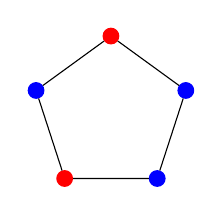
\begin{tikzpicture}[baseline]
          \foreach \x/\c in {0/red,1/blue,2/blue,3/red,4/blue} {
            \node[draw, \c, circle, fill=\c, inner sep=2pt]
                at ({sin(360 * \x / 5)}, {cos(360 * \x / 5)}) (\x) {};
          }
          \draw[] (0) -- (1) -- (2) -- (3) -- (4) -- (0);
    \end{tikzpicture} &
    G[c] &={} 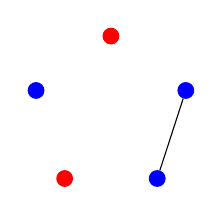
\begin{tikzpicture}[baseline]
        \foreach \x/\c in {0/red,1/blue,2/blue,3/red,4/blue} {
          \node[draw, \c, circle, fill=\c, inner sep=2pt]
              at ({sin(360 * \x / 5)}, {cos(360 * \x / 5)}) (\x) {};
        }
        \draw[] (1) -- (2);
    \end{tikzpicture}
  \end{align*}
\end{example*}
These are related to colourings as follows.
\begin{note*}
  $G$ is $t$-colourable iff $G$ is $t$-colourable with defect 0 iff $G$ is
  $t$-colourable with clustering 1.
\end{note*}
The two notions of colouring are related as follows.
\begin{proposition}
  \listhack
  \begin{enumerate}[label=(\arabic*)]
    \item If $G$ is $t$-colourable with clustering $k$ then $G$ is
      $t$-colourable with defect $k-1$.

    \item If $G$ is $t$-colourable with defect $k$,
      then $G$ is $t(k+1)$-colourable.
  \end{enumerate}
\end{proposition}
\begin{proof}
  \leavevmode\vspace{-0.5em}
  \begin{enumerate}[label=(\arabic*)]
    \item Easy.

    \item If $c$ is a $t$-colouring of $G$ with defect $k$,
      then each monochromatic component of $G$ is $(k+1)$-colourable
      (by degeneracy); so for each monochromatic component with colour $\kappa$,
      properly $(k+1)$-colour it with colours
      $(\kappa, 0), (\kappa, 1), \ldots, (\kappa, k)$: this gives a $t(k+1)$
      colouring of $G$. \qedhere
  \end{enumerate}
\end{proof}
This implies that if $\mathcal G$ is a class of graphs, the following are equivalent:
\begin{itemize}
  \item there exists $t$ such that every $G\in\mathcal G$ is $t$-colourable;
  \item there exists $t,k$ such that every $G\in\mathcal G$ is $t$-colourable
    with clustering $k$; and
  \item there exists $t,k$ such that every $G\in\mathcal G$ is $t$-colourable
    with defect $k$.
\end{itemize}
\begin{theorem}
  If $d\geq 0$, then every graph $G$ is
  $\left(\floor{\frac{\Delta(G)}{d+1}}+1\right)$-colourable with defect $d$.
\end{theorem}
\begin{proof}
  Let $k = \floor{\frac{\Delta(G)}{d+1}}+1$, and let $c$ be a $k$-colouring of
  $G$ with as few monochromatic edges as possible.
  Suppose $c$ does not have defect $d$, so there is a vertex $v$ with at least
  $d+1$ neighbours of the same colour.

  This implies $v$ has at most $\deg(v) - (d+1)\leq\Delta(G) - (d+1)$ neighbours
  with a different colour than $c(v)$, so there is some colour $\kappa$
  appearing on at most $\frac{\Delta(G) - (d+1)}{k-1}$ neighbours of $v$ in $G$.
  By the minimality in the choice of $c$, we must have
  $\frac{\Delta(G)-(d+1)}{k-1}\geq d+1$, since otherwise we could recolour $v$
  with colour $\kappa$ and reduce the number of monochromatic edges.
  This gives
  \begin{align*}
    \Delta(G) - (d+1)\geq(k-1)(d+1)\implies k\leq\frac{\Delta(G)}{d+1}
  \end{align*}
  but $k = \floor{\frac{\Delta(G)}{d+1}}+1$, which is a contradiction.
\end{proof}
\begin{theorem}[Dujmovi\'c, Esperet, Monn, Wood]
  For all $t$, there exists $c$ so that every $K_t$-minor-free graph is
  $(t-1)$-colourable with clustering $c$ where $c = c(t)$ is large.
\end{theorem}
\begin{proof}
  Relies on graph minor structure theorem, so proof very much omitted.
\end{proof}
\begin{theorem}[Van den Heuvel, Wood]
  If $K_t\not\leq G$ then
  \begin{itemize}
    \item $G$ is $(t-1)$-colourable with defect $t-2$; and
    \item $G$ is $(2t-2)$-colourable with clustering $\ceil{\half(t-2)}$.
  \end{itemize}
\end{theorem}
We first need some definitions and lemmas to be able to prove this.
\begin{definition*}[Spanner]
  A \vocab{spanner} for a set $X\subseteq V(G)$ is a minimal set $S\supseteq X$
  such that $G[S]$ is connected.
\end{definition*}
Because for finite objects we have minimal objects, if $H$ is any connected
induced subgraph of $G$ containing $X$, then $H$ contains a spanner for $X$.
\begin{definition*}[$k$-spanner]
  A \vocab[spanner!k-spanner@\2]{$k$-spanner} is a spanner for a set $X$ with
  $|X|\leq k$.
\end{definition*}
These objects have degree bounds.
\begin{proposition}
  If $S$ is a $k$-spanner, then $\Delta(G[S])\leq k$.
\end{proposition}
\begin{proof}
  Let $v$ be a vertex of degree strictly greater than $k$ in $G[S]$.
  Let $T$ be a spanning tree of $G[S]$ containing all edges at $v$.

  Since $T - v$ has more than $k$ components, some component $H$ of $T - v$
  contains no vertex in $X$.
  Now $G[S] - V(H)$ is connected (as $T - H$ is a spanning tree), and contains
  $X$.
  This contradicts minimality.
\end{proof}
\begin{definition*}
  We say sets $X,Y\subseteq V(G)$ are \vocab{adjacent} if $G$ has an edge from
  $X$ to $Y$.
\end{definition*}
The following is the main lemma.
\begin{lemma}
  If $t\geq 4$, $K_t\not\leq G$, then $V(G)$ has a partition $(S_1,\ldots,S_n)$
  such that:
  \begin{itemize}
    \item each $S_i$ is a $(t-2)$-spanner in $G$; and
    \item for each $\ell\in\{1,\ldots,n\}$ and each component $C$ of
      $G - (S_1\cup\ldots\cup S_\ell)$ the sets in $\{S_1,\ldots, S_\ell\}$
      that are adjacent to $C$ are pairwise adjacent to each other.
  \end{itemize}
\end{lemma}
\begin{proof}
  Choose $S_1 = \{v\}$ for some $v$.
  It is enough to show that, for all $S_1,\ldots,S_k$ satisfying the conditions,
  if $S_1\cup\cdots\cup S_k\neq V(G)$, then we can find $S_{k+1}$ such that
  $S_1,\ldots,S_{k+1}$ satisfy the conditions.

  \lecture{Tue Nov 07}%
  Let $C$ be a component of $G - (S_1\cup\cdots\cup S_k)$.
  If there are at least $t-1$ sets in $S_1,\ldots,S_k$ that are adjacent to $C$,
  then $G$ has a $K_t$-minor (contract all edges inside $C$ and the sets
  adjacent to $C$).
  Therefore there are at most $t-2$ sets in $S_1,\ldots,S_k$ adjacent to $C$.
  Call them $S_{i_1},\ldots,S_{i_h}$ where $h\leq t-2$.
  For each $1\leq j\leq h$, let $x_j$ be a vertex in $C$ adjacent to some vertex
  in $S_{i_j}$.
  Let $S_{k+1}$ be a spanner for $\{x_1,\ldots,x_h\}$.
  We show that $S_{k+1}$ is a ``valid'' choice
  (i.e. it satisfies the inductive hypothesis).

  Let $C'$ be a component of $G - (S_1\cup\cdots\cup S_{k+1})$, and let $C_0$
  be the component of $G - (S_1\cup\cdots\cup S_k)$ containing $C'$.
  If $C_0\neq C$, then (since there is no edge from $C_0$ to $C$),
  $C'$ is not adjacent to $S_{k+1}$, and the sets in $\{S_1,\ldots,S_k\}$
  adjacent to $C'$ are adjacent to $C_0$, and so by the inductive
  hypothesis, are adjacent to each other.

  If $C = C_0$, a similar argument works (using the construction of $S_{k+1}$).
\end{proof}
\begin{corollary}
  For the $S_1,\ldots,S_n$ chosen in the lemma, for each $1\leq\ell\leq n$,
  the sets in $\{S_1,\ldots,S_{\ell-1}\}$ adjacent to $S_\ell$ are pairwise
  adjacent, and there are at most $t-2$ of them.
\end{corollary}
\begin{proof}
  Left as an exercise to the reader.
\end{proof}
\begin{corollary}
  If $K_t\not\leq G$ and $t\geq 4$ then $G$ is $t-1$-colourable with defect $t-2$.
\end{corollary}
\begin{proof}
  For $i = 1, \ldots, n$, we colour all vertices in $S_i$ with colour not
  assigned to any of the at most $t-2$ sets in $S_1,\ldots,S_{i-1}$ that are
  adjacent to $S_i$.
  By construction, no two adjacent $S_i$ receive the same colour,
  and by the lemma, each $S_i$ is a $(t-2)$-spanner so has $\Delta(S_i)\leq t-2$
  (and the monochromatic components are all $S_i$).
\end{proof}
\begin{remark*}
  The same partition can be used to show that $G$ is $(2t-2)$-colourable with
  clustering $\frac{k}{2}$ as each spanner is 2-cluster-colourable.
\end{remark*}
\subsection{Girth and Chromatic Number}
\begin{theorem}[Erd\H{o}s]\th\label{thm:girth-chi-unbounded}
  \mnote[-8em]{The intuition here is girth is ``downwards monotone'', i.e. as you add
  more edges, you would expect girth to decrease, but chromatic number is
  ``upwards monotone'', i.e. if you add more edges, you would expect chromatic
  number to increase.}%
  For all $g,t\geq 1$, there is a graph with girth at least $g$ (i.e. the
  shortest cycle has length at least $g$) and chromatic number at least $t$.
\end{theorem}
The ``obvious'' idea (adding the expected chromatic number and number
of short cycles) doesn't work.
Additionally, the proof actually shows a stronger result by bounding the
independence number $\alpha(G)$, which gives $\chi(G)\geq\frac{|V(G)||}{\alpha(G)}$.
We need the following lemma.
\begin{lemma}\th\label{lem:girth-chi-unbounded-helper}
  If $g,t\geq 3$ and $n\geq\max(14t,(4g)^g)$, then there is a graph $G$ on $n$
  vertices with $\alpha(G)\leq\frac{n}{2t}$ and with at most $\frac{n}{2}$
  cycles of length strictly less than $g$.
\end{lemma}
We can now prove the theorem.
\begin{proof}[Proof of \th\ref{thm:girth-chi-unbounded}]
  Take such a $G$.
  Let $X$ be a set containing at least 1 vertex from every cycle with strictly
  less than $g$ vertices with $|X|\leq\frac n 2$.
  Then $G - X$ has girth at least $g$ by construction and
  \[
    \chi(G-X)\geq\frac{|V(G-X)|}{\alpha(G-X)}\geq\frac{n - \nicefrac n 2}{\alpha(G)}
    \geq\frac{\nicefrac n 2}{\nicefrac n{2t}} = t. \qedhere
  \]
\end{proof}
To prove the lemma, we need the following corollary of Markov's inequality.
\begin{corollary}[Corollary of Markov's inequality]
  If $X$ is a $\bN$-valued random variable with finite expectation then
  $\bP(X\geq 2E[X])\leq\half$.
\end{corollary}
\begin{proof}
  \leavevmode\vspace{-0.5em}
  \begin{align*}
    \bE[X] &= \sum_{i\geq 0}\bP(X=i)\cdot i \\
           &= \sum_{i < 2\bE[X]}i\cdot\bP(X=i) + \sum_{i\geq 2\bE[X]}i\cdot\bP(X=i) \\
           &\geq 0 + 2\bE[X]\sum_{i\geq 2\bE[X]}\bP(X=i) \\
           &= 2\bE[X]\cdot\bP(X\geq 2\bE[X]).
  \end{align*}
  Also, note you can change the ``2'' for any natural $k$ and the result still
  holds.
\end{proof}
We can now prove the lemma.
\begin{proof}[Proof of \th\ref{lem:girth-chi-unbounded-helper}]
  Let $p = n^{\frac 1 g - 1}$ and let $G$ be chosen by including each edge
  independently with probability $p$ (i.e. $G = G_{n,p}$).
  Then
  \begin{align*}
    \bE[\#\text{ cycles of length }<g]
    &\leq\sum_{i=3}^{g-1} n^i p^i \tag{the number of $i$ cycles is at most $n^i$} \\
    &= \sum_{i=3}^{g-1}(np)^i = \sum_{i=1}^{g-1}n^{\frac i g} \\
    &\leq gn^{\frac{g-1}{g}} \\
    &\leq\frac n 4 \tag{because $n\geq (4g)^g$}
  \end{align*}
  so $\bP(\#(<g)\text{-cycles}\geq\frac n 2)\leq\half$ by Markov.

  We now consider the expected number of independent sets of size at least
  $\floor{\frac{n}{2t}}$.
  \begin{align*}
    \bE\left[\#\floor{\frac{n}{2t}}-\text{ind sets}\right]
    &= \binom{n}{\floor{\nicefrac{n}{2t}}}(1-p)^{\binom{\floor{\nicefrac{n}{2t}}}{2}}\\
    &\leq\left(\frac{en}{\nicefrac{n}{2t}}\right)^{\nicefrac{n}{2t}}
      \cdot e^{-p\cdot\nicefrac{n^2}{4t^2}}
    \tag{using $1-p\leq e^{-p}$ and $\binom{n}{k}\leq\left(\frac{en}{k}\right)^k$} \\
    &\leq (2te)^{\nicefrac{n}{2t}}\cdot
        e^{-n^{\nicefrac{1}{g}-1}\cdot\nicefrac{n^2}{4t^2}} \\
    &\leq e^{\frac{n}{2t}\log(2t)}\cdot e^{-n^{\frac 1 g + 1}\cdot\frac{1}{4t^2}} \\
    &=\exp\left(n\cdot\frac{\log(2t)}{2t} - \frac{n^{1+\frac 1 g}}{4t^2}\right) \\
    &=\exp\left(n\left(\frac{\log 2t}{2t} - \frac{1}{4t^2}\cdot n^{\nicefrac 1 g}\right)\right) \\
    &\leq\exp(-n) \tag{for $n$ large enough} \\
    &\leq e\inv < \nicefrac 1 2
  \end{align*}
  so
  \[
    \bP\left(\exists(<g)\text{-cycle or a }\floor{\frac{n}{2t}}\text{-ind set}\right)
    < \nicefrac 1 2 + \nicefrac 1 2 = 1
  \]
  so there is some $G$ where neither occurs.
\end{proof}
\begin{question*}
  When is $\chi$ large?
\end{question*}
Possibly because there is a large clique, but the girth-chromatic number
number says this cannot be the only reason.
The girth chromatic number also says that this generalizes to any set of
graphs (that are not forests), because there exists a graph that has
girth larger than the minimum girth of all graphs in said set.

More intuitively, ``large girth'' implies ``tree-like'',
so the girth-chromatic number theorem says that you can have
``locally tree-like'' graphs with high chromatic number.

\begin{theorem}[Rodl 1977]
  \mnote{I found out during office hours this might not be a completely accurate
  restatement of the theorem. Also, the triangle-free subgraph is not
  necessarily induced; there's actually counterexamples if you force it to be
  induced.}
  There is a function $f(m,t)$ so that if $G$ is a graph with
  $\chi(G)\geq f(m,t)$, the either $G$ has a $K_m$-subgraph,
  or $G$ has a triangle-free subgraph $H$ with $\chi(H)\geq t$.
\end{theorem}

This theorem answers the above question: a graph has large chromatic number
because either the graph contains a clique, or a triangle-free subgraph.

\begin{conjecture}
  There is a function $f(m,t)$ so that if $G$ is a graph with
  $\chi(G)\geq f(m,t)$, the either $G$ has a $K_m$-subgraph,
  or $G$ has a subgraph $H$ with girth at least $g$ and $\chi(H)\geq t$.
\end{conjecture}
\subsection{Edge Colourings}
\lecture{Thu Nov 09}
\begin{question*}
  What if we want to colour the \underline{edges} of $G$?
\end{question*}
Let $\chi'(G)$ be the minimum number of colours required to colour the edges of
$G$ so that adjacent edges get different colours.
\begin{note*}
  $\chi'(G) = \chi(L(G))$ where the \vocab{line graph} $L(G)$ has
  $V(L(G)) = E(G)$ and vertices (edges) are adjacent if they are adjacent in $G$.
\end{note*}
We have the following bounds.
\begin{proposition}
  \leavevmode\vspace{-1em}
  \[
    \chi'(G) = \chi(L(G))\leq\Delta(L(G)) + 1 \leq 2\Delta(G) - 1
  \]
\end{proposition}
The above can be strengthened in certain cases by using Brook's Theorem.
\begin{proposition}
  $\chi'(G)\geq\Delta(G)$.
\end{proposition}
\begin{proof}
  Obvious.
\end{proof}
The following lemma will allow us to (inductively) prove Vizing's theorem.
\begin{lemma}[Schrijver]
  \mnote{Induction and maximum degree don't work well together because removing
  parts of the graph might not drop maximum degree, so instead we want
  hypotheses about local properties of the graph.}
  Let $k\geq 0$.
  If $v$ is a vertex of a graph $G$ such that
  \begin{itemize}
    \item $G - v$ is $k$-edge colourable;
    \item all vertices in $N(v)\cup\{v\}$ have degree at most $k$ in $G$; and
    \item at most one neighbour of $v$ has degree $k$;%
      \rmnote{I think this condition is to force the gap that allows for
      the parity argument to go through.}
  \end{itemize}
  then $G$ is $k$-edge colourable.
\end{lemma}
\begin{proof}
  The lemma is vacuously true for $k = 0$.
  Suppose $k\geq 1$ and the result holds for $k - 1$.
  We may assume $d(v) > 0$. Let $z$ be a neighbour of $v$ of largest degree;
  so $\deg(x)\leq k-1$ for all $x\in N(v)\setminus\{z\}$.

  Let $G^+$ be obtained from $G$ by adding ``pendant edges'' to all vertices
  in $N(v)$ until $z$ has degree $k$ and all other neighbours of $v$ have degree
  $k-1$.

  Note that, since $G - v$ is $k$-edge colourable, so is $G^+-v$;
  it thus suffices to argue that $G^+$ is $k$-edge colourable.
  \rmnote{Be careful when assuming the object is a maximal / simpler one in general
  induction arguments, because it can break very delicate induction hypotheses.}%
  We may assume, therefore, that $d(x) = k-1$ for all $x\in N(v)\setminus\{z\}$;
  and that $d(z) = k$.

  For each $k$-edge colouring $c : E(G-v)\to [k]$, and each $i\in[k]$ let
  $D^c_i = \{x\in N(v) : \text{colour }i\text{ is missing at }x\}$.
  \mnote{I.e. pick $c$ so it minimizes the distance of $\{D_i^c\}$ from the
  average / variance.}%
  Choose a colouring $c$ so that $\sum_{i=1}^k |D_i^c|^2$ is a small as possible.
  There are then two cases.
  \begin{itemize}
    \item \textbf{Case 1:} $|D_a^c| = 1$ for some $a$.

      Let $u\in N(v)$ be the unique vertex such that no edge at $u$ has colour
      $a$.
      Let $E_a = \{e\in E(G - v) : c(e) = a\}$.
      Let $G' = G - (E_a\cup\{uv\})$.
      By construction, $d_{G'}(x) = d_G(x) - 1$ for all $x\in \{v\}\cup N_G(v)$,
      and also, $G' - v$ is $(k-1)$-edge colourable (using $c$), so inductively,
      $G'$ is $(k-1)$-edge-colourable.
      Assigning colour $a$ to the edges in $E_a\cup\{uv\}$ gives a $k$-edge
      colouring of $G$.

    \item $|D_i^c|\neq 1$ for all $i$.

      Note that
      \begin{align*}
        \sum_{i=1}^k |D_c^i|
        &= \sum_{i=1}^k\#\{\text{vertices in }N(u)\text{ missing }i\} \\
        &= \sum_{x\in N(v)}\#\{\text{colours missing at }x\} \\
        &= 2(\deg(v)-1)+1
      \end{align*}
      because $d_{G-v}(x) = k - 2$ for all $x\neq z$, and $d_{G-v}(z) = 1$.
      Thus the sum of the $|D_i^c|$ is odd, and the average size is
      \[
        \frac{\sum_{i=1}^k |D_i^c|}{k} = \frac{2d(v) - 1}{k} \leq\frac{2k-1}{k} < 2.
      \]
      It follows that there exists $a$ such that $D_a^c = \varnothing$ and $b$
      such that $|D^c_b|$ is odd; note that $|D^c_b|\neq 1$;
      let $s = |D_b^c|\geq 3$.

      Let $H$ be the spanning subgraph of $G$ containing only the edges with
      colour $a$ or $b$.
      $H$ has maximum degree at most 2, and by construction, an odd number of
      neighbours of $v$ have degree 1 in $H$.
      It follows that $H$ has a path component $P$ with exactly one end, $u$,
      in $N(v)$.
      Since $N_a^c = \varnothing$, we know colour $a$ is present at $u$,
      and colour $b$ is missing.
      Let $c'$ be the colouring obtained from $c$ by switching the colours of
      every edge in $P$ between $a\leftrightarrow b$.

      \mnote{Alternatively, reduce to the first case.}%
      By construction, $D_a^{c'}= \{u\}$ and $D_b^{c'} = D_b^c\setminus\{u\}$
      and $D_i^{c'} = D_i^c$ for all $i\neq a,b$.
      Therefore
      \begin{align*}
        \sum_{i=1}^k|D_i^{c'}|^2
        &= \sum_{i=1}^k |D_i^c|^2 + (|D_a^{c'}|^2 - |D_a^c|^2) + (|D_b^{c'}|^2 - |D_b^c|^2) \\
        &= \sum_{i=1}^k |D_i^c|^2 + (1^2 - 0^2) + ((s-1)^2 - s^2) \\
        &< \sum_{i=1}^k |D_i^c|^2
      \end{align*}
      since $s\geq 3$. \qedhere
  \end{itemize}
\end{proof}
\begin{theorem}[Vizing's Theorem]
  If $G$ is a graph then $\chi'(G)\in\{\Delta(G),\Delta(G)+1\}$.
\end{theorem}
\begin{proof}
  It suffices to show that $\chi'(G)\leq k = \Delta(G) + 1$
  (because the lower bound follows trivially).
  Let $G$ be a vertex-minimal counterexample, $v\in V(G)$.
  Now $\chi'(G-v)\leq\Delta(G-v)+1\leq\Delta(G) + 1 = k$ by the inductive hypothesis.

  The hypotheses of the previous lemma with $k = \Delta(G) + 1$ are trivially
  satisfied, so $G$ is $k$-edge colourable.
\end{proof}
\begin{remark*}
  If $G$ satisfies $\chi'(G) = \Delta(G)$ then it is \vocab{class 1},
  and if $\chi'(G) = \Delta(G) + 1$ then it is \vocab{class 2}.
\end{remark*}
Distinguishing the two is hard.
\begin{theorem}[Holger 1981]
  Deciding whether $G$ is class 1 or 2 is NP-complete, even when $G$ is 3-regular.
\end{theorem}
\begin{proof}
  Proof omitted.
\end{proof}
\begin{theorem}[Vizing + Gupta]
  For multigraphs $G$, $\chi'(G)\leq\Delta(G) + m(G)$ where $m(G)$
  is the maximum edge multiplicity.
\end{theorem}
\begin{proof}
  Proof omitted.
\end{proof}
\begin{theorem}[Berget + Fournier 1991]
  If $G$ is a multigraph and $m(G)\leq t$ and
  \[
    \{x\in V(G) : d(x) = \Delta(G)\text{ and }x\text{ is on an edge with multiplicity }t\}
  \]
  is a stable set then $\chi'(G)\leq\Delta(G) + t - 1$.
\end{theorem}
This implies that if in $G$ the set $\{x\in V(G) : d(x) = \Delta(G)\}$ is
a stable set, then $G$ is class 1.
It also implies the previous theorems.

\begin{theorem}[Csabu, K\"uhn, Lo, Osthus, Treglown 2016]
  There exists $n_0$ such that if $G$ is a regular graph with an even number of
  vertices with an even number $n\geq n_0$ of vertices,
  and degree at least $\frac n 2$, then $\chi'(G) = \Delta(G)$.
\end{theorem}
\begin{proof}
  Proof omitted.
\end{proof}
\begin{theorem}[Konig 1916]
  If $G$ is bipartite then $\chi'(G) = \Delta(G)$.
\end{theorem}
\begin{proof}
  Induct on $|E(G)|$: let $e = uv\in E(G)$ and consider an $\Delta(G)$-edge
  colouring of $G - e$.
  It follows that $u$ is not incident to colour $a$ and $v$ colour $b$,
  where if $a = b$, then assigning $e$ colour $a$ gives a $\Delta(G)$-colouring
  of $E$.

  Otherwise, $a\neq b$, and consider a maximal path $P$ starting at $u$ in
  $G - e$ alternating between edges of colour $a$ and $b$.
  Because bipartite graphs do not have odd cycles, the colours along $P$
  can be swapped without causing any difficulties, and then $e$ can be coloured
  with colour $b$.
\end{proof}
\end{document}
